\documentclass[12pt]{article}
\usepackage[utf8]{inputenc}
\usepackage{amsmath}
\usepackage[pdftex]{hyperref}
\usepackage{graphics}
\usepackage[brazil]{babel}
\usepackage{empheq,amsmath}
\usepackage{mathtools}
\usepackage{natbib}
\usepackage{indentfirst}
\usepackage{graphicx}
\usepackage{svg}
\usepackage[hyphenbreaks]{breakurl}




\usepackage{float}
\usepackage[left=2.00cm,right=2.00cm,top=2.00cm,bottom=2.00cm]{geometry}

\begin{document}
\date{}
\title{Modelagem Matemática da Dinâmica da Epidemia do COVID-19 na Alemanha}
\author{Eduardo Corrêa Araujo}
\maketitle

\begin{abstract}
    O presente trabalho tem o objetivo de propor um modelo compartimental extendido do tipo SEIR para analisar a dinâmica da epidemia de COVID-19 na Alemanha. Os principais objetivos são analisar o impacto das medidas de controle da epidemia na taxa de contágio e  quais são as principais diferenças entre a primeira e a segunda onda da epidemia no país indicadas pelo modelo.
\end{abstract}

\section{Introdução}

 Em dezembro de 2019, os primeiros casos de COVID-19 foram confirmados em Wuhan, a sétima maior cidade da China. No início de Janeiro de 2020, o SARS-Cov-2, vírus causador da COVID-19, que ficou conhecido como o novo coronavírus, se espalhou para outras regiões da China e do mundo. Em 11 de março, em virtude do alto potencial de espalhamento e severidade observados a Organização Mundial da Saúde (OMS) declarou que a situação da COVID-19 poderia ser caracterizada como uma pandemia. Em 13 de Março de 2020, o diretor geral da  OMS declarou que a Europa tinha se tornado o epicentro da pandemia do COVID-19 \cite{OMS}. 

O primeiro caso confirmado de COVID-19 na Alemanha foi reportado no final de Janeiro de 2020. Em 1 de Março, mais de 100 casos já haviam sido confirmados. A primeira morte confirmada foi reportada em 9 de março de 2020 \cite{goetz2020covid}. Na Alemanha, o Instituto Robert Koch (RKI) divulga diariamente relatórios sobre a situação da pandemia no país \cite{RKI}.

Em 16 de Março, o governo iniciou as primeiras medidas de combate ao espalhamento da doença: escolas, jardins de infância e universidades foram fechadas. Em 17 de Março, as lojas foram fechadas (exceto as com artigos essenciais, como mercados e farmácias), além da imposição de restrições de viagens. Em 22 de Março, foi implementada uma política de distanciamento social: as pessoas foram avisadas para saírem apenas se necessário e em grupos de no máximo 2 pessoas, caso essas não morassem na mesma casa, além do fechamento de restaurantes e outros provedores de serviço, como cabeleireiros \cite{goetz2020covid, wieland2020flatten}.

Em 20 de abril, após uma estabilização do aumento do número de casos, houve a reabertura de muitas lojas menores que 800 $m^2$ e alguns outros serviços. Em 06 de maio, houve um maior número de flexibilizações, todas as lojas podiam reabrir sendo mantido o distanciamento e o uso de máscara, além da permissão da reabertura gradual dos colégios. Se o número de casos aumentasse consideravelmente, essas medidas poderiam ser revistas e os estabelecimentos teriam que fechar novamente \cite{wieland2020flatten, bbc06.05, tg06.05}. Nesse cenário, esse fechamento seria voltado para as regiões com o aumento expressivo do número de casos.

Em 15 de junho, foi permitida a entrada de turistas da União Européia  e do Reino Unido, Islândia, Noruega, Liechtenstein e Suíça \cite{dw}. Em 01 de julho, foi liberada a entrada de pessoas oriundas de alguns outros países \cite{sgvi}. No início de agosto, apesar do aumento dos casos, a maior parte das escolas começaram a reabrir na Alemanha \cite{fortuneschool}.

No relatório publicado no dia 03 de setembro de 2020, pelo RKI, sobre a situação da epidemia na Alemanha foi destacado que o número de casos tem estabilizado desde meados de julho. Nesse relatório foi destacado também que a diferença de mortalidade entre os casos reportados observada tem sido menor, em função do fato de que, no momento, a maior parte das infecções está ocorrendo na parcela mais jovem da população, sendo os principais surtos relacionados a viagens e reuniões de famílias \cite{RKI}.

No entanto, como destacado no relatório publicado no dia 03 de outubro de 2020, pelo RKI, o número de casos começou a subir a partir de meados de setembro também no grupo de pessoas mais velhas. Esse aumento levou a um crescimento expressivo do número de mortos em outubro. Esta situação levou a imposição de novas medidas de controle da epidemia na Alemanha, no dia 2 de Novembro, com o objetivo de controlar o avanço do número de casos e mortes. Nas novas medidas, escolas e lojas permanecerão funcionando, porém, bares, restaurantes e academias deverão ser fechados até que os casos se estabilizem novamente, além disso é recomendado que as pessoas se reunam apenas em grupos pequenos de no máximo 10 pessoas e de no máximo duas famílias diferentes \cite{2lock1, 2lock2}.

 Veja na Tabela \ref{medidas} um resumo das medidas adotadas na Alemanha.

\begin{table}[h]
\label{medidas}
\centering
\begin{small}
\caption{Medidas Adotadas na Alemanha durante a pandemia do COVID-19} 
\begin{tabular}{|p{0.5cm}|p{10cm}|p{4.5cm}|}
\hline
             & Medida Adotada & Data\\
\hline
1& Escolas, jardins de infância e universidades foram fechadas.          & 16 de Março de 2020. \\
\hline
2& Fechamento de comércio não essencial e restrições de viagem.          & 17 de Março de 2020. \\
\hline

3& Política de distanciamento social, as pessoas foram avisadas para saírem apenas se necessário e em grupos de no máximo 2 pessoas, caso essas não morassem na mesma casa, mantendo um distanciamento de 1.5 m. Serviços como restaurantes e salões de cabeleireiros foram fechados.  & 22 de Março de 2020. \\

\hline

4 & Reabertura de lojas menores que 800 $m^2$ e serviços. Alguns dias depois foi imposta a obrigatoriedade do uso de máscaras no transporte público e em lojas. & 20 de Abril de 2020. \\

\hline
5 & Maior número de flexibilizações, lojas maiores que 800 $m^2$ poderiam reabrir, além da permissão da abertura gradual dos colégios. & 06 de Maio de 2020. \\

\hline

6 & Fim das restrições de viagem para os países da União Européia (UE) e alguns outros países. A partir dessa data foi ocorrendo uma flexibilização dos países, cujo habitantes poderiam viajar para a Alemanha. & 15 de Junho de 2020.\\
\hline 

7 & Reabertura das escolas na Alemanha. & 01 de Agosto de 2020.\\
\hline

8 & Fechamento de bares, restaurantes e academias. & 02 de Novembro de 2020. \\
\hline
\end{tabular}
\end{small}
\end{table}

A Figura \ref{graphmedidas} representa a data de adoção das medidas e a curva de casos acumulados. Na figura há uma diferenciação entre primeira e segunda onda de casos no dia 15 de junho. Esta postura foi adotada pois posteriormente o modelo apresentado neste trabalho será estimado separadamente para cada uma das ondas. Essa data foi adotada na divisão pois como pode ser observado na Tabela 1, em 15 de junho houve o fim de algumas restrições de viagem. Além disso, foi utilizado como referência o comportamento da curva que mostra uma tendência de crescimento após essa data. 

\begin{figure*}[h!]
    \label{graphmedidas}
    \centering
    \includesvg[scale = 0.6]{Medidas_adotadas.svg}
    \caption{Data da aplicação das medidas adotadas na Alemanha em contraste com a curva de casos acumulados.}
\end{figure*}

Com o aumento do número de casos na Alemanha foram aplicados diversos modelos matemáticos na tentativa de compreender a dinâmica da doença a longo prazo e quais são as suas principais características. Dentre os trabalhos publicados, podemos destacar o modelo  compartimental do tipo SEIR com mortos de Goetz and Heidrich que inclui uma função variável para a taxa de contágio, analisando o impacto das medidas adotadas na Alemanha na redução da taxa de contágio \cite{goetz2020covid}. Também o modelo proposto por Liu e seus colaboradores, cujo principal objetivo é analisar o impacto dos indivíduos não identificados com poucos ou nenhum sintomas na dinâmica da doença \cite{liu2020predicting}. Além disso, há o trabalho de Barbarossa e seus colaboladores, no qual é proposto um modelo estruturado por idades e é analisado o impacto de possíveis políticas de controle da doença \cite{barbarossa2020modeling}. Ademais, há o trabalho de Kergassner e seus colaboladores, em que, através de um modelo SIR espacial com um compartimento a mais para os quarentenados, é analisado como as interações entre as diferentes regiões da Alemanha impactam na dinâmica do COVID-19 no país.
 
%%%%%%%%%%%%%%%%%%%%%%%%%%%%%%%%%%%%%%%%%%%%%%%%%%%%%%%%%%%%%%
\section{Metodologia}
\subsection{Obtenção dos dados}

Os dados utilizados nesse trabalho foram retirados da plataforma \url{https://ourworldindata.org/}. Para capturar os dados foi criado um script em python disponível em \url{https://github.com/eduardocorrearaujo/Avaliacoes-MM4-/blob/master/Avalia\%C3\%A7\%C3\%A3o\%20A2/Obtencao_dos_dados.ipynb}.

Utilizando os dados disponíveis, foi possível plotar os gráficos abaixo. 

\begin{figure}[h!]
    \centering
    \includesvg[scale = 0.4]{curvas.svg}
    \caption{Na primeira linha, a esquerda temos a curva de casos acumulados e a direita a curva de novos casos. Na segunda linha, a esquerda a curva de óbitos acumulados e a direita a curva de novos óbitos.}
    \label{fig:my_label}
\end{figure}


\newpage
\subsection{Modelo SEIR extendido}
Nesse trabalho é proposto um modelo extendido do tipo SEIR para analisar a dinâmica do espalhamento da COVID-19 na Alemanha.

O modelo adotado  divide a população em 7 classes diferentes: $S$ representa os indivíduos suscetíveis, que ainda não foram infectados, $E$ representa os indivíduos expostos, que estão no período de incubação, já que há conhecimento clínico de que a doença possui um período de incubação. Esses indivíduos são aqueles que foram infectados, mas ainda não desenvolveram nenhum sintoma e não estão infecciosos. Passado o período de incubação,   o modelo assume duas possibilidades distintas: o indivíduo pode ir para $I_D$ que engloba os indivíduos identificados pelo sistema de saúde que tem sintomas mais graves da doença ou para $I$ que representa os indivíduos que não foram identificados e possuem sintomas mais leves ou nenhum sintoma. A possibilidade do indivíduo ser identificado ou não é representada no modelo pelo parâmetro $p$. Se o indivíduo não for identificado, é considerado que ele tem sintomas leves ou não tem nenhum sintoma, logo, assumimos que ele não irá vir a óbito, se recuperando com uma taxa $\gamma$  e indo para $R$, que representa os recuperados. Se o indivíduo for identificado, assumimos que ele deve ter sintomas mais graves da doença. Logo, para esses indivíduos existem duas possibilidades, eles podem se recuperar com uma taxa $\gamma_D$ indo para o compartimento $R_D$, que representa os recuperados diagnosticados ou acabar falecendo com uma probabilidade $\delta$ indo para o compartimento $D$, que representa os óbitos. 


Além disso, no modelo é considerado que os indivíduos identificados são isolados, assim, o modelo considera um fator de correção $q$ para a sua infectividade, visto que como são isolados eles não tem o mesmo potencial de infectar outros indivíduos, mas ainda podem infectar pessoas nos hospitais, ou pessoas na própria família pensando nos indivíduos que estão isolados em domicílio, incluindo também os indivíduos que desrespeitam o isolamento.  Foi feita a divisão entre identificados e não identificados visto que muitos indivíduos tem sintomas leves ou não possuem sintomas da doença, assim, acabam não sendo identificados e isolados, tendo contato com um número muito maior de pessoas, o que aumenta o seu potencial de infecção. Veja na Figura 6 o diagrama do modelo e na Tabela 2 o significado de cada um dos parâmetros apresentados no diagrama.

\begin{figure*}[h!]
    \centering
    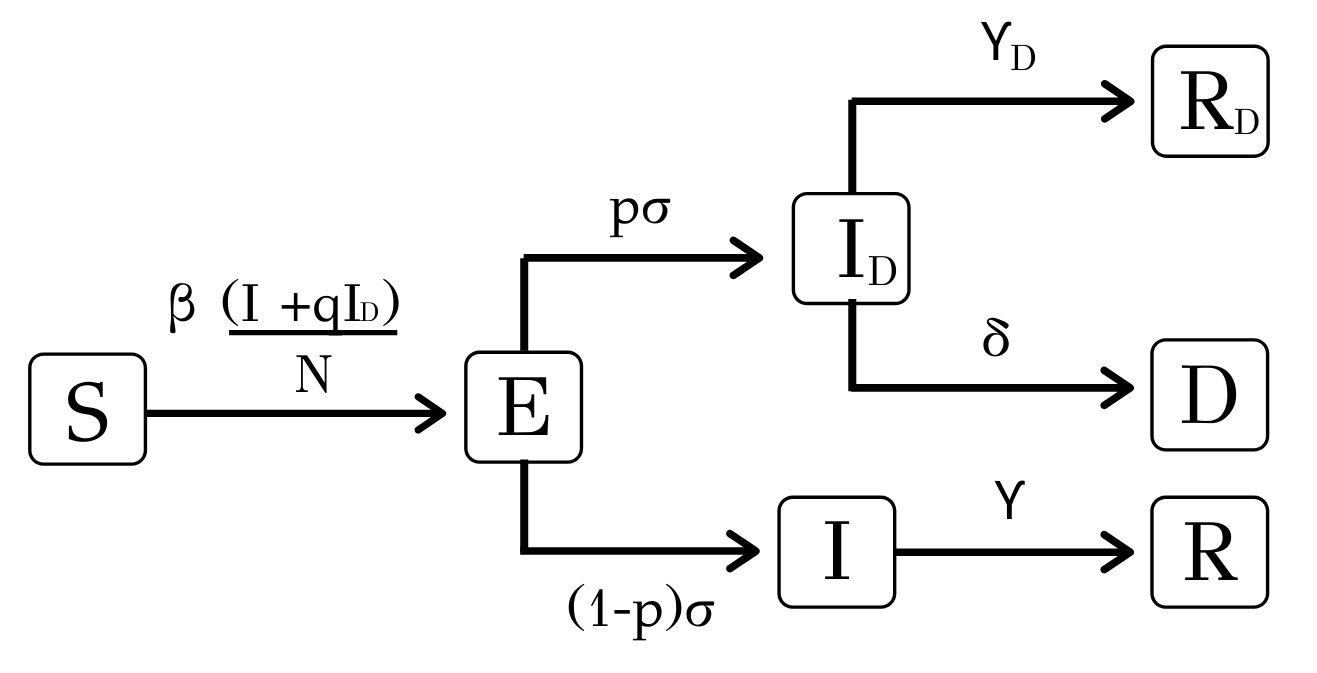
\includegraphics[scale = 0.3]{fluxograma.png}
    \caption{Diagrama do modelo SEIARD - SEIR extendido.}
\end{figure*}


O modelo é definido pelo seguinte sistema de Equações Diferenciais Ordinárias:

\begin{center}
$$
\begin{cases}
\dot S = \cfrac{-\beta_i(t)S(I + qI_D)}{N}. \\
\dot E = \cfrac{\beta_i(t)S(I + qI_D)}{N} - \sigma E. \\
\dot {I} = (1-p)\sigma E - \gamma I.\\
\dot {I_D} = p\sigma E - \gamma_DI_D - \cfrac{\gamma_D \delta_i (t)}{1 - \delta_i(t)}I_D.\\
\dot {R} = \gamma I.\\
\dot {R_D} = \gamma_DI_D.\\
\dot {D} = \cfrac{\gamma_S \delta_i(t)}{1 - \delta_i(t)}I_D.

\end{cases}
$$
\end{center}

\noindent Com condições iniciais: $$S(t_0) = S_0 > 0, E(t_0) = E_0 \geq 0, I(t_0) = I_0 \geq 0, I_D(t_0) = {I_D}_0 > 0,$$
$$R(t_0) = R_0 \geq 0, R_D(t_0) = {R_D}_0 \geq 0, D(t_0) = D_0 \geq 0.$$ Esse modelo possui a propriedade de conservação da massa, sendo assim, $S + E + I + I_D + R + R_D + D = N$, ou seja, a população é sempre constante, o modelo não considera efeitos de imigração, emigração, natalidade e mortalidade, é considerada apenas a mortalidade da doença.

É importante ressaltar que a mortalidade dos indivíduos diagnosticados poderia ser representada por um taxa de remoção $\theta I_D$, porém seguindo \cite{keeling2011modeling} ela foi representada pelo termo $\frac{\delta \gamma_D }{1 - \delta} I_D$ onde $\delta$ representa a probabilidade de um indivíduo infectado morrer antes de se recuperar. Foi utilizada essa formulação pois ela facilita a interpretação biológica do parâmetro e sua estimação a partir dos dados.

\begin{table}[h]
\centering
\begin{small}
\caption{Parâmetros do modelo} \label{Tabela1}
\begin{tabular}{|p{2cm}|p{14cm}|}
\hline
            Parâmetro & Significado \\
\hline
$t_0$ & tempo inicial. \\
\hline
$S_0$ & Número de indivíduos suscetíveis em $t_0$.\\
\hline 
$E_0$ & Número de indivíduos expostos em $t_0$.\\
\hline 
$I_0$ & Número de indivíduos não identificados (com poucos ou nenhum sintomas) em $t_0$.\\
\hline 
$I_{D_0}$ & Número de indivíduos identificados em $t_0$.\\
\hline 
$R_0$ & Número de indivíduos recuperados não identificados em $t_0$.\\
\hline 
$R_{D_0}$ & Número de indivíduos recuperados identificados em $t_0$.\\
\hline 
$D_0$ & Número de indivíduos mortos em $t_0$.\\
\hline 
$\beta(t)$ & Taxa de contágio, no modelo é representada por uma função dependente do tempo. \\
\hline
$q$ & Correção para a infectividade dos indivíduos identificados, isso é feito em virtude do protocolo de isolamento para esses indivíduos o que diminui sua probabilidade de infectar outras pessoas.\\
\hline
$N$ & População da Alemanha. \\
\hline
$\sigma$ & inverso do tempo médio de incubação do vírus. \\
\hline
$p$ & representa a taxa de identificação dos indivíduos infectados.\\
\hline
$\gamma$ & inverso do tempo médio de recuperação dos indivíduos não identificados. \\
\hline
$\gamma_D$ & inverso do tempo médio de recuperação dos indivíduos identificados.\\
\hline
$\delta(t)$ & taxa de mortalidade da doença, que é expressa por uma função dependente do tempo. \\
\hline
\end{tabular}
\end{small}
\end{table}



O modelo foi fitado separadamente para cada uma das ondas, considerando a primeira onda do dia 28/01 ao dia 15/01 e a segunda onda do dia 15/01 ao dia 26/11 como exposto na Figura 
\ref{graphmedidas}. Em cada uma das ondas foi utilizado uma formulação ligeiramente diferente para $\beta(t)$ e $\delta(t)$. Por essa razão esses parâmetros são indicados com um subíndice $i$, para a primeira onda teremos $\beta_1(t)$ e $\delta_1(t)$ e para a segunda onda $\beta_2(t)$ e $\delta_2(t)$.

\subsection{Função $\beta_i(t)$}

Para a escolha da função $\beta(t)$ a primeira postura adotada foi considerar essa função como uma função degrau constante, cujos degraus eram definidos com base nas medidas adotadas na Alemanha, seguindo o que foi feito em \cite{goetz2020covid}.

Utilizando essa abordagem, foi realizada uma estimação prévia dos parâmetros do modelo, utilizando o método dos mínimos quadrados, considerando apenas a primeira onda e considerando a função $\beta(t)$ como: 

$$ \beta_1(t) =
\begin{cases}
\beta_0 : \text{t $<$ 22 de Março.} \\
\beta_1 : \text{22 de Março $<$ t $<$ 20 de Abril.}\\
\beta_2 : \text{20 de Abril $<$ t $<$ 06 de Maio.} \\
\beta_3 : \text{06 de Maio $<$ t $<$ 15 de Junho.} \\
\end{cases}$$


Para essa estimação prévia o resultado obtido está representado na Figura \ref{beta1teste}.
\begin{figure}[h!]
    \centering
    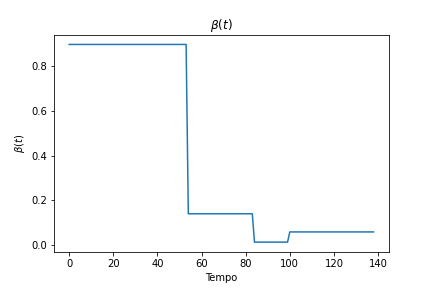
\includegraphics[scale = 0.6]{beta1_teste.png}
    \caption{Os parâmetros estimados foram: $b_0 = 0.898, b_1 = 0.139, b_2= 0.011, b_3 = 0.057.$}
    \label{beta1teste}
\end{figure}

Como o comportamento obtido foi muito similar a um decrescimento logístico essa função degrau foi substituída por uma outra função que reproduz esse comportamento de decrescimento e é contínua e diferenciável. Assim, a função $\beta(t)$, para primeira onda ficou definida por: 

$$\beta_1(t) = \cfrac{\beta_0 - \beta_1}{1 + e^{-k(x_0 - t)}} + \beta_1, $$

\noindent onde $x_0$ reprenta o instante em que a taxa de contágio começou a diminuir, $k$ representa a intensidade da sua redução e $\beta_0$ e $\beta_1$ estão relacionados ao valor inicial e final da taxa de contágio. 

Para a função $\beta_2(t)$, relacionada a segunda onda (15/06 a 26/11) a abordagem foi análoga. Primeiramente foi considera a função:

$$ \beta_2(t) =
\begin{cases}
\beta_4 : \text{t $<$ 01 de Agosto.} \\
\beta_5 : \text{01 de Agosto $<$ t $<$ 02 de Novembro.}\\
\beta_6 : \text{t $>$ 02 de Novembro.} \\
\end{cases}$$


\noindent O resultado obtido da estimação desses parâmetros está representado na Figura \ref{beta2teste} . 

\begin{figure}[h!]
    \centering
    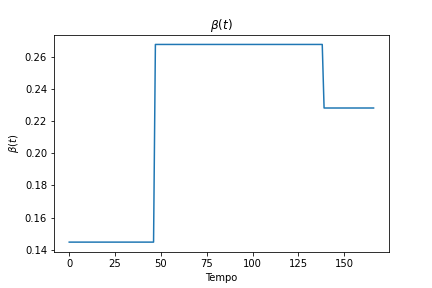
\includegraphics[scale = 0.6]{beta2_teste.png}
    \caption{Os parâmetros estimados foram: $b_4 = 0.145, b_5 = 0.268, b_6= 0.228. $}
    \label{beta2teste}
\end{figure}

Como o comportamento da função é similar a um crescimento logístico ela foi substituída pela função: 

$$\beta_2(t) = \cfrac{\beta_4 - \beta_5}{1 + e^{k(x_0 - t)}} + \beta_5. $$

\noindent onde $x_0$ reprenta o instante em que a taxa de contágio começou a crescer, $k$ representa a intensidade do crescimento e $\beta_4$ e $\beta_5$ estão relacionados ao valor inicial e final da taxa de contágio. 

É importante ressaltar que para ambos os casos foram comparados os resultados de se utilizar as funções degrau ou as funções logísticas e as últimas conseguiram representar melhor a dinâmica da doença.


\subsection{Função $\delta_i(t)$}

Para a primeira onda foi considerado um valor constante para mortalidade, $\delta_1(t) = \delta$. Já para a segunda onda, foi considerado uma função dependente do tempo, pois a segunda onda teve características diferentes da primeira, as quais, influenciam no valor da mortalidade, entre elas temos:

\begin{itemize}
    \item aumento do número de testes;
    \item aumento do conhecimento médico sobre a melhor forma de tratar a doença;
    \item diferença na idade dos infectados. A segunda onda da epidemia na Alemanha tem como característica que a maior parte dos infectados fazem parte da parcela mais jovem da população, que tem uma mortalidade menor.
\end{itemize}
Por esses motivos foi adotado um descrecimento logístico para a mortalidade expresso por: 

$$\delta_2(t) = \cfrac{\delta_0 - \delta_1}{1 + e^{\mu(dat - t)}} + \delta_1,$$

\noindent em que $\delta_0$ e $\delta_1$ estão relacionados a mortalidade inicial e final, $\mu$ a intensidade do decrescimento e $dat$ a data em que a mortalidade começou a diminuir.



\subsection{Pontos de equilíbrio do modelo}

Para analisar os pontos de equilíbrio do modelo podemos analisar apenas as equações $(S,E,I,I_D)$ já que o sistema não depende das outras variáveis. Fazendo isso, encontramos que  o modelo não possui nenhum ponto de equilíbrio endêmico e possui um único ponto de equilíbrio livre de doença expresso por: $(S, E, I,I_D, R, R_D, D) = (\overline{s}, 0,0,0,0,0,0,)$ , $\overline{s} > 0$. Podemos tentar analisar a estabilidade deste ponto de equilíbrio através da análise do sinal dos autovalores da matriz jacobiana do sistema. Para esse sistema a matriz jacobiana é:

\begin{center}
$J(S,E, I, I_D)$=
$\begin{pmatrix} -\cfrac{\beta}{N} (I + qI_D) & 0 & -\cfrac{\beta S}{N}  & -\cfrac{\beta q S}{N} \\
-\cfrac{\beta}{N} (I + qI_D) & -\sigma &  \cfrac{\beta S}{N} & \cfrac{\beta q S}{N}\\
0 & (1-p)\sigma & -\gamma & 0 \\
0 & p \sigma & 0 & -\cfrac{\gamma_D}{ 1 - \delta}
\end{pmatrix}.$
\end{center}

No ponto de equilíbrio livre de doença:
\begin{center}
$J(\overline{s},0, 0, 0)$=
$\begin{pmatrix} 0 & 0 & -\cfrac{\beta \overline{s}}{N}  & -\cfrac{\beta q \overline{s}}{N} \\
0 & -\sigma &  \cfrac{\beta \overline{s}}{N} & \cfrac{\beta q \overline{s}}{N}\\
0 & (1-p)\sigma & -\gamma & 0 \\
0 & p \sigma & 0 & -\cfrac{\gamma_D}{ 1 - \delta}
\end{pmatrix}.$
\end{center}

Como um dos autovalores da matriz é nulo, não podemos definir se o ponto de equilíbrio é estável ou não. Isto pois a matriz jacobiana é apenas uma aproximação do sistema, ela possui um erro associado, o qual pode tornar esse autovalor positivo ou negativo, o que influencia diretamente na estabilidade do ponto.



\subsection{Análise Dimensional do Modelo}
Como visto anteriormente, o modelo é definido pelo seguinte sistema de equações diferenciais ordinárias:
\begin{center}
$$
\begin{cases}
\dot S = \cfrac{-\beta(t)S(I + qI_D)}{N}. \\
\dot E = \cfrac{\beta(t)S(I+ qI_D)}{N} - \sigma E .\\
\dot {I} = (1-p)\sigma E - \gamma I.\\
\dot {I_D} = p \sigma E - \gamma_DI_D - \cfrac{\gamma_D \delta (t)I_D}{1 - \delta(t)}.\\
\dot {R} = \gamma I.\\
\dot {R_D} = \gamma_DI_D.\\
\dot {D} = \cfrac{\gamma_D \delta (t)I_D}{1 - \delta(t)}.
\end{cases}
$$
\end{center}


Vamos assumir que a escala de tempo, $t$, do modelo é expressa em dias. Sabemos que os lados esquerdos das equações acima tem dimensão $[M]/[T]$, onde $M$ representa a massa e $T$ o tempo. Assim, na primeira equação concluímos que $S, I, I_D, N$ tem dimensão $[M]$, $\beta(t)$ tem dimensão $[T]^{-1}$ e $q$ é adimensional. Na segunda equação, concluí-se que $\sigma$ tem dimensão $[T]^{-1}$. Na terceira equação concluí-se que $\gamma$ tem dimensão $[T]^{-1}$ e $p$ é adimensional. Na quarta equação concluí-se que $\gamma_D$ tem dimensão $[T]^{-1}$ e $\delta(t)$ é adimensional. 

Para tornar o sistema adimensional, primeiro no tocante a massa, podemos assumir que 

$S^* = \cfrac{S}{N}$, logo $S^*$ é adimensional, derivando ambos os lados em relação ao tempo, encontramos:
$$\cfrac{dS^*}{dt} = \cfrac{dS}{dt} \cdot \cfrac{1}{N} = \cfrac{-\beta(t)S(I + qI_D)}{N \cdot N}.$$
Procedendo do mesmo modo com as outras equações, encontramos que:
$$E^* = \cfrac{E}{N} \implies \cfrac{dE^*}{dt} = \cfrac{dE}{dt} \cdot \cfrac{1}{N} = \cfrac{\beta(t)S(I + qI_D)}{N \cdot N} - \cfrac{\sigma E}{N},$$
$$I^* = \cfrac{I}{N} \implies \cfrac{dI^*}{dt} = \cfrac{dI}{dt} \cdot \cfrac{1}{N} = \cfrac{ (1-p)\sigma E - \gamma I}{N},$$
$$I_D^* = \cfrac{I_D}{N} \implies \cfrac{dI_D^*}{dt} = \cfrac{dI_D}{dt} \cdot \cfrac{1}{N} = \cfrac{ p\sigma E - \gamma_DI_D - \cfrac{\gamma_D\delta (t)I_D}{1 - \delta(t)}}{N},$$
$$R^* = \cfrac{R}{N} \implies \cfrac{dR^*}{dt} = \cfrac{dR}{dt} \cdot \cfrac{1}{N} = \cfrac{\gamma I}{N},$$
$$R_D^* = \cfrac{R-D}{N} \implies \cfrac{R_D^*}{dt} = \cfrac{dR_D}{dt} \cdot \cfrac{1}{N} = \cfrac{\gamma_DI_D}{N},$$
$$D^* = \cfrac{D}{N} \implies \cfrac{dD^*}{dt} = \cfrac{dD}{dt} \cdot \cfrac{1}{N} = \cfrac{\gamma_D \delta (t)I_D}{N(1 - \delta(t))}.$$



Substituindo $ S^* = \cfrac{S}{N}, E^* = \cfrac{E}{N}, I^* = \cfrac{I}{N},I_D^* = \cfrac{I_D}{N},R^* = \cfrac{R}{N},R_D^* = \cfrac{R_D}{N},D^* = \cfrac{D}{N} $ nas equações que encontramos para $\dot S^*,\dot E^*,\dot I^*,\dot I_D^*,\dot R^*, \dot R_D^*, \dot D^*$, o modelo adimensional no tocante a massa é:
\begin{center}
$$
\begin{cases}
\dot S^* = -\beta(t)S^*(I^* + qI_D^*). \\
\dot E^* = \beta(t)S^*(I^* + qI_D^*) - \sigma E^*. \\
\dot {I^*} = (1-p)\sigma E^* - \gamma I^*.\\
\dot {I_D^*} = p\sigma E^* - \gamma_DI_D^* - \cfrac{\gamma_D \delta (t)I_D^*}{1 - \delta(t)}.\\
\dot {R^*} = \gamma I^*.\\
\dot {R_D^*} = \gamma_DI_D^*.\\
\dot {D^*} = \cfrac{\gamma_D \delta (t)I_D^*}{1 - \delta(t)}.

\end{cases}
$$
\end{center}

\noindent onde $S^* + E^* +I^*+I_D^*+R^*a+R_D^*+D^* = \cfrac{N}{N} = 1.$

Resta agora adimensionalizar em relação ao tempo. Se $t^* = \gamma t$, note que $t^*$ é adimensional. Derivando ambos os lados em relação a $t^*$ encontramos:
$$t^* = \gamma t \implies \cfrac{dt^*}{dt^*} = \gamma \cfrac{dt}{dt^*} \implies \cfrac{dt}{dt^*} = \cfrac{1}{\gamma}.$$

Para a primeira equação do sistema adimensional em relação a massa, aplicando a regra da cadeia, temos que:
$$\cfrac{dS^*}{dt^*} = \cfrac{dS^*}{dt} \cdot  \cfrac{dt}{dt^*} = -\beta(t)S^*(I^* + qI_D^*) \cdot \cfrac{1}{\gamma}.$$

Aplicando a mesma análise para cada uma das outras equações do sistema obtemos o seguinte sistema adimensional:

\begin{center}
$$
\begin{cases}
\cfrac{dS^*}{dt^*} = \cfrac{-\beta(t)S^*(I^* + qI_D^*)}{\gamma}. \\
\cfrac{dE^*}{dt^*}  = \cfrac{\beta(t)S^*(I^* + qI_D^*) - \sigma E^* }{\gamma}.\\
\cfrac{dI^*}{dt^*}  = \cfrac{(1-p)\sigma E^* - \gamma I^*}{\gamma}.\\
\cfrac{dI_D^*}{dt^*}  = \cfrac{p\sigma E^* - \gamma_DI_D^*}{\gamma} - \cfrac{\gamma_D \delta (t)I_D^*}{\gamma(1 - \delta(t))}.\\
\cfrac{dR^*}{dt^*}  = I^*.\\
\cfrac{dR_D^*}{dt^*}  = \cfrac{\gamma_DI_D^*}{\gamma}.\\
\cfrac{dD^*}{dt^*}  = \cfrac{\gamma_D \delta (t)I_D^*}{\gamma(1 - \delta(t))}.

\end{cases}
$$
\end{center}


\subsection{Cálculo do $R_0$}

O $R_0$ é definido como o número médio de infecções causadas por um único indivíduo infeccioso introduzido em uma população totalmente imune \cite{randolph2020herd}.
Para o cálculo do $R_0$ do modelo foi utilizado o método da matriz de próxima geração, o qual está descrito em \cite{van2002reproduction}. Após aplicar este método para o modelo o resultado encontrado para o $R_0$ foi: 

$$R_0 = \cfrac{\beta [ \gamma_D (1-p) + \gamma (1 - \delta)pq]}{\gamma \gamma_D}.$$

Apenas a formulação do $R_0$ nos permite retirar informações importantes sobre o impacto dos parâmetros do modelo no espalhamento da doença. Na Figura \ref{sensR_0}, há dois gráficos representando a sensibilidade do $R_0$ aos parâmetros $p$ e $q$ do modelo. Para criar esse gráfico foram fixadas os outros parâmetros deixando apenas variar o parâmetro de interesse na análise.


\begin{figure}[h!]
    \centering
    \includesvg[scale = 0.5]{sens_do_R_0.svg}
    \caption{O gráfico da esquerda representa a sensibilidade do $R_0$ ao parâmetro $p$ e o gráfico da direita a sensibilidade ao parâmetro $q$. Para gerar os gráficos foram fixados: $\beta = 0.3, \gamma = 1/9, \gamma_D = 1/9, p = 0.5, q = 0.3 $, variando $p$ de $0$ a $1$ no gráfico da esquerda e $q$ de $0$ a $1$ no gráfico da direita.}
    \label{sensR_0}
\end{figure}

Note que na Figura \ref{sensR_0}, no gráfico da esquerda, quanto maior o valor de $p$, menor o $R_0$. Como $p$ representa a taxa de detecção dos indivíduos infectados, a qual está relacionado com a testagem, o gráfico está nos indicando que quanto mais efetivo for a testagem na identificação dos indivíduos infectados mais difícil será da doença se espalhar.

Já o gráfico da direita Figura \ref{sensR_0}, que mostra a sensibilidade do $R_0$ em relação ao $q$, nos mostra que quanto maior o valor de $q$, maior será o valor de $R_0$. Assim, como $q$ é o parâmetro relacionado a efetividade do isolamento dos indivíduos identificados, quanto menos efetiva for o seu isolamento maior será o valor de $q$ e mais facilmente a doença irá se espalhar, pois o $R_0$ será maior.

A partir do $R_0$ podemos também definir o $R_t$, o número de reprodução efetivo, que é definido como o número médio de infecções causadas por um único indivíduo infeccioso  introduzido em uma população parcialmente imune \cite{randolph2020herd}. Para o modelo deste trabalho ele é representado por: 
$$R_t(t) = \cfrac{\beta [ \gamma_D (1-p) + \gamma (1 - \delta)pq]}{\gamma \gamma_D}\cdot \cfrac{S(t)}{N}.$$

O $R_t (t)$ é muito importante, pois considerando uma doença em que o indivíduo após infectado adquire imunidade permanente, ele nos permite estimar quando a população atingirá a imunidade de rebanho que é o ponto, a partir do qual, naturalmente o número de infectados tende a diminuir, que é o ponto em que $R_t (t) < 1$.

\subsection{Análise da sensibilidade}

Foi realizada uma análise da sensibilidade do modelo aos parâmetros para determinar os parâmetros mais relevantes, que devem ser ajustados e quais podemos considerar constantes utilizando, por exemplo, valores da literatura para fixá-los. Para a análise da sensibilidade foi utilziado o método de Sobol's \cite{saltelli2010variance}. Este método retorna índices de sensibilidade que podem ser de vários tipos. Neste trabalho serão considerados em análise o índice de primeira ordem, expresso por:
$$S_i = \cfrac{V_i}{Var(Y)},$$
que representa a contribuição de cada parâmetro $V_i$ para a variância da saída do modelo $(Var(Y))$. Há também os índices de ordem total expressos por:
$$S_{Ti}={\frac {E_{{\textbf {X}}_{\sim i}}\left(\operatorname {Var} _{X_{i}}(Y\mid \mathbf {X} _{\sim i})\right)}{\operatorname {Var} (Y)}}=1-{\frac {\operatorname {Var} _{{\textbf {X}}_{\sim i}}\left(E_{X_{i}}(Y\mid \mathbf {X} _{\sim i})\right)}{\operatorname {Var} (Y)}},$$
que medem a contribuição de cada parâmetro para a variância de saída do modelo.

Como o objetivo deste trabalho é analisar as curvas de casos acumulados e óbitos, foi analisado a sensibilidade dos parâmetros em relação ao valor do pico da curva $I_D$ (infectados diagnosticados), ao valor do pico da curva $D$ (óbitos) e ao valor da soma dos picos de $I_D$ e $D$. Como são utilizados modelos diferentes para cada uma das ondas, foi realizada duas análises de sensibilidade.

\subsubsection{ Sensibilidade do modelo da primeira onda}

A Figura \ref{sens1onda} representa os gráficos da sensibilidade dos parâmetros em relação a cada um dos valores acima. Analisando os gráficos fica claro que os parâmetros menos infuentes para as saídas desejada são $\gamma$, $k$, $x_0$, $\sigma$. Por essa razão, $k$ foi fixado como $k = 0.25$, já que o variando o seu valor seu impacto não era significativo na saída do modelo, quanto ao $x_0$, ele será fitado pelo modelo tendo uma margem de alguns dias ao redor do dia 22 de Março, dia em que a Alemanha adotou as primeiras medidas mais rígidas de combate a pandemia. Quanto aos parâmetros $\gamma$ e $\sigma$, como estão relacionados a características da doença, serão utilizados valores da literatura, será fixado $\sigma = 1/5$ aproximando o valor apresentado em \cite{li2020early} e $\gamma = 1/6$ seguindo \cite{barbarossa2020modeling}.
\begin{figure}[h!]
    \includesvg[width=0.5\textwidth]{SensibilidadeaoI_D.svg}
    \includesvg[width=0.5\textwidth]{SensibilidadeaoI_DeD.svg}
    \includesvg[width=0.5\textwidth]{Sensibilidadeao_D.svg}
    
    \caption{A figura superior a esquerda representa a sensibilidade dos parâmetros do modelo ao valor pico de $I_D$ a figura da direita representa a sensibilidade ao valor da soma do pico de $I_D$ e $D$, a figura inferior a esquerda representa a sensibilidade ao valor do pico de $D$. Os parâmetros no eixo $x$ do gráfico são, da esquerda para direita, $p$, $q$, $\beta_0$, $\beta_1$, $k$, $x_0$, $\gamma$, $\gamma_D$, $\delta$, $\sigma$ respectivamente.}
    \label{sens1onda}
\end{figure}

\subsubsection{ Sensibilidade do modelo da segunda onda}

A Figura \ref{sens2onda} representa os gráficos da sensibilidade dos parâmetros em relação a cada um dos valores descritos anteriormente. Analisando os gráficos fica claro que os parâmetros menos influentes para as saídas desejada são $\gamma$, $k$, $x_0$, $mu$ $\sigma$, $dat$. Logo, assim como foi feito para a primeira onda, foi fixados $k = 0.25$, e $\sigma = 1/5$, $\gamma = 1/6$, como o parâmetro $\mu$ representa o decrescimento e  não gera muita influência na saída do modelo foi fixado como $\mu = 0.25$, assim como $k$. O parâmetro $dat$ será fitado para incluir a data em que a mortalidade começa a diminuir.



\begin{figure}[h!]
    \includesvg[width=0.5\textwidth]{Sensibilidade_2I_D_D.svg}
    \includesvg[width=0.5\textwidth]{Sensibilidade_2I_D.svg}
    \includesvg[width=0.5\textwidth]{Sensibilidade_2_D.svg}
    
    \caption{A figura superior a esquerda representa a sensibilidade dos parâmetros do modelo ao valor do pico de $I_D$ a figura da direita representa a sensibilidade ao valor da soma do pico de $I_D$ e $D$, a figura inferior a esquerda representa a sensibilidade ao valor do pico de $D$. Os parâmetros no eixo $x$ do gráfico são, da esquerda para direita, $p$, $q$, $\beta_5$, $\beta_6$, $k$, $x_0$, $\gamma$, $\gamma_D$, $\delta_0$, $\delta_1$, $\mu$, $dat$, $\sigma$, respectivamente.}
    \label{sens2onda}
\end{figure}


\section{Resultados} 

Para verificar a adequação do modelo aos dados foi utilizado o método dos mínimos quadrados implementado utilizando o pacote lmfit \cite{LMFIT} da linguagem de programação Python. 

Para  a primeira onda, como descrito na análise de sensibilidade, foram fixados $\gamma = 1/6, \ \sigma~=~1/5$ e  $k=0.25$. Os outros parâmetros foram ajustados, dentro de um intervalo específico. Para o parâmetro $p$ foi considerado um intervalo de $[0,0.8]$, já que é natural que no decorrer da epidemia nem todos os indivíduos sejam identificados. O parâmetro $q$ foi considerado em um intervalo de $[0,0.5]$, considerando que os indivíduos isolados tem um potencial de infecção no mínimo $50\%$ menor quando comparado com os indivíduos que não estão isolados. Os parâmetros $\beta_0$ e $\beta_1$ foram considerados variando no intervalo $[0,1]$, o parâmetro $x_0$ foi considerado variando no intervalo $[45,65]$, pois este intervalo inclui a data das primeiras medidas de controle da epidemia e o parâmetro $\delta$ foi considerado variando no intervalo $[0.048, 0.052]$, pois ao realizar simulações, se considerado um intervalo superior ou inferior a curva dos mortos era pior representada. Para o $\gamma_D$ foi considerado um intervalo de $[1/7, 1/14]$, já que segundo estudos a maior parte dos indivíduos perdem a infecciosidade cerca de $10$ dias após o início dos sintomas  \cite{RKI2}, assim foi fixado um intervalo ao redor de $10$ dias para encontrar o valor ótimo de $\gamma_D$.


Para realizar a estimação dos parâmetros foi utilizado a curva de casos acumulados, pois, como foi considerado desde o dia com o primeiro caso reportado, as condições iniciais do modelo foram fixadas em: $S_0 = 83019999, \ E_0 = 0, \ I_0 = 0, \ {I_D}_0 = 1, \ R=0, \ {R_D}_0 =0$ e $D_0 = 0$. A Figura \ref{fitting1onda} representa o resutado obtido utilizando o método dos mínimos quadrados, o gráfico da esquerda é referente a estimação da curva de casos acumulados e o da direita a curva de óbitos. 

\begin{figure}[h!]
    \centering
    \includesvg[scale = 0.425]{fitting.svg}
    \includesvg[scale = 0.425]{comp_obitos.svg}
    \caption{O gráfico a esquerda representa a comparação da curva de casos estimada pelo modelo e a curva de casos acumulados real e o gráfico a direita representa a comparação entre a curva de óbitos estimada e a curva de óbitos real.}
    \label{fitting1onda}
\end{figure}

Para verificar a precisão do modelo foi utilizada como métrica de erro a mediana do erro relativo, para cada valor dos dados foi calculado:
$$e_i = \cfrac{ \vert (f(t_i, \theta) - y_{t_i})\vert}{y_{t_i}}, $$

em que $f(t_i, \theta)$ representa a curva estimada pelo modelo e $y_{t_i}$ os dados. Após calcular $e_i$ para todos os pontos foi selecionado o valor da mediana dos valores de $e_i$ como uma estimativa do erro do modelo. 
Para a curva de casos acumulados o erro estimado foi de $0.007 $ e para a curva de óbitos acumulados o erro estimado foi de  $0.03$. A baixa precisão da estimativa da curva de óbitos, se comparada com a de casos, muito provavelmente está relacionada ao fato de estar sendo ajustada apenas a curva de casos acumulados. Assim, uma possibilidade de melhoria seria utilizar uma outra formulação para a função a ser minimizada (nesse caso está sendo utilizada a formulação clássica do método dos mínimos quadrados) incluindo os mortos ou adicionando um peso a eles. Pretendo implementar essa melhoria futuramente no trabalho. O resultado dos parâmetros fitados está representado na Tabela \ref{resparam1}. 

\begin{table}[h]
\label{resparam1}
\centering
\begin{small}
\caption{Resultado da estimação dos parâmetros}
\begin{tabular}{|p{2cm}|p{2cm}|p{2cm}|p{2cm}|p{2cm}|p{2cm}|p{2cm}|}
\hline
 $p$ & $q$ & $\beta_0$ & $\beta_1$ & $x_0$ & $\gamma_D$ & $\delta$\\
\hline
 $0.40$ & $0.42$ & $0.95$ & $0.08$ & $56.65$ & $0.07$ & $0.048$\\
\hline
\end{tabular}
\end{small}
\end{table}


Utilizando os parâmetros estimados foi calculado o valor do $R_t(t)$, número de reprodução efetivo da doença, no decorrer do tempo. O seu gráfico está representado na Figura \ref{rt1}. 

\begin{figure}[h!]
    \centering
    \includesvg[scale = 0.5]{Rt.svg}
    \caption{Estimativa do $R_t(t)$ - número de reprodução efetivo.}
    \label{rt1}
\end{figure}

Ainda não há um consenso para o valor do $R_0$ da doença, estudos estimam que ele pode estar no intervalo $[2.2, 4.71] $ ou ser até mesmo maior do que 6 \cite{barbarossa2020modeling}. Para os parâmetros estimados do modelo o $R_0$ calculado foi de $5.63$. 

Observando o gráfico do $R_t$ na Figura \ref{rt1} vemos que o $R_t(t)$ tende a diminuir entre os dias $50$ e $70$, o que é condizente com as medidas adotadas. Além disso, note que o $R_t(t)$ fica abaixo de $1$ próximo ao dia $70$, indicando que a epidemia estaria sobre controle. Estes resultados são consequência da imposição de $\beta_1(t)$ como uma função logística decrescente. Os parâmetros estimados resultaram no gráfico de $\beta_1(t)$ da Figura \ref{beta1t}.

\begin{figure}[h!]
    \centering
    \includesvg[scale = 0.5]{beta1.svg}
    \caption{Variação da taxa de contágio $\beta_1(t)$ no decorrer do tempo.} 
    \label{beta1t}
\end{figure}

Para verificar a efetividade do modelo em descrever o comportamento da primeira onda preditivamente foi realizado um teste estimando os parâmetros do modelo utilizando $30$ dias anteriores ao fim da primeira onda e comparando a curva estimada para esses $30$ dias e qual foram os dados. O resultado está ilustrado na Figura \ref{comp1onda}. Os parâmetros obtidos estão na Tabela \ref{Tabcomp1onda}.

\begin{table}[h]
\centering
\begin{small}
\caption{Resultado da estimação dos parâmetros, estimando com 30 dias a menos} \label{Tabcomp1onda}
\begin{tabular}{|p{2cm}|p{2cm}|p{2cm}|p{2cm}|p{2cm}|p{2cm}|p{2cm}|}
\hline
 $p$ & $q$ & $\beta_0$ & $\beta_1$ & $x_0$ & $\gamma_D$ & $\delta$\\
\hline
 $0.21$ & $0.49$ & $0.91$ & $0.08$ & $56.07$ & $0.072$ & $0.048$\\
\hline
\end{tabular}
\end{small}
\end{table}

\begin{figure}[h!]
    \centering
    \includesvg[scale = 0.40]{fittingcomp.svg}
    \includesvg[scale = 0.40]{fittingcompdepois.svg}
    \caption{O gráfico da esquerda representa a curva estimada para os casos acumulados utilizando $30$ dias a menos. O gráfico da direita representa a comparação entre a curva simulada nos próximos $30$ dias para o modelo e os dados. }
    \label{comp1onda}
\end{figure}

Para o gráfico da esquerda da Figura \ref{comp1onda} o erro estimado foi de $0.03$ e para o da direita o erro estimado foi de $0.01$.

%%%%%%%%%%%%%%%%%%%%%%%%%%%%%%%%%%%%5 2 ONDA %%%%%%%%%%%%%%%%%%%%%%%%%%%%%%%%%%%%%

Para a segunda onda, assim como descrito na análise de sensibilidade e feito para a primeira onda, foram fixados $\gamma = 1/6, \ \sigma = 1/5, \ k = 0.25 \ , \mu = 0.25$. Os outros parâmetros foram ajustados, dentro de um intervalo específico. Para o parâmetro $p$ e $q$ foi considerado um intervalo igual ao da primeira onda. Os parâmetros $\beta_5$ e $\beta_6$ foram considerados variando no intervalo $[0,1]$, o parâmetro $x_0$ foi considerado variando no intervalo $[30,100]$, para incluir o período de reabertura das escolas, para o $\delta_0$ foi considerado variando no intervalo $[0.01,0.048]$ e para o $\delta_1$  o intervalo de $[0.09,0.015]$ pois ao realizar simulações, se considerado um intervalo superior ou inferior a curva dos mortos era pior representada, para o $dat$ foi considerado um intervalo de $[0,30].$ Para o $\gamma_D$ foi considerado um intervalo de $[1/7, 1/14]$ já que segundo estudos a maior parte dos indivíduos perdem a infecciosidade cerca de $10$ dias após o início dos sintomas  \cite{RKI}. Assim, foi fixado um intervalo ao redor de $10$ dias para encontrar o valor ótimo de $\gamma_D$.
Para realizar a estimação dos parâmetros foi utilizado a curva de casos acumulados, assim como na primeira onda. Foram fixadas como condições iniciais o último valor de cada uma das curvas estimadas para a primeira onda. A Figura \ref{fitting2onda} representa o resultado obtido utilizando o método dos mínimos quadrados, o gráfico da esquerda é referente a estimação da curva de casos acumulados e o da direita a curva de óbitos.
Para o gráfico da esquerda da Figura \ref{fitting2onda} referente a curva de casos acumulados o erro estimado foi de $0.02$, já para o gráfico da direita referente a curva de mortos o erro estimado foi de $0.04$.

\begin{figure}[h!]
    \centering
    \includesvg[scale = 0.425]{fitting2onda.svg}
    \includesvg[scale =0.425]{Comparando_obitos2.svg}
    \caption{O gráfico a esquerda representa a comparação da curva de casos estimada pelo modelo e a curva de casos acumulados real e o gráfico a direita representa a comparação entre a curva de óbitos estimada e a curva de óbitos real.}
    \label{fitting2onda}
\end{figure}

Os parâmetros estimados pelo modelo estão representados na Tabela 5.

\begin{table}[h!]
\label{resuparams2}
\centering
\begin{small}
\caption{Resultado da estimação dos parâmetros da segunda onda} 
\begin{tabular}{|p{1.5cm}|p{1.5cm}|p{1.5cm}|p{1.5cm}|p{1.5cm}|p{1.5cm}|p{1.5cm}|p{1.5cm}|p{1.5cm}|}
\hline
 $p$ & $q$ & $\beta_5$ & $\beta_6$ & $x_0$ & $\gamma_D$ & $\delta_0$ & $\delta_1$ & $dat$\\
\hline
 $0.38$& $0.5$& $0.30$ & $0.24$ & $77.31$ & $0.143$ & $0.048$ & $0.009$ & $21.21$ \\
\hline
\end{tabular}
\end{small}
\end{table}

Analisando o resultado dos parâmetros estimados para a segunda onda é imediato perceber que os parâmetros $p$ e $\delta_0$ foram muito similares aos resultados obtidos na primeira onda. O resultado de $q$, condizente com o valor máximo do intervalo em que ele foi ajustado, está indicando que os individuos sintomáticos, mesmo isolados, estão tendo uma taxa de contágio de mais de $50\%$ do valor da taxa do indivíduos infectados que não foram identificados e isolados. Esse resultado pode estar relacionado com a infecção causada por esses indivíduos quando pré-sintomáticos, já que, se tem conhecimento de que os indivíduos infectados e com sintomas podem infectar cerca de $1-2$ dias antes do início dos sintomas \cite{he2020temporal}, por essa razão, uma possibilidade para verificar a validade desse resultado é incluir os pré-sintomáticos na dinâmica da doença e analisar o impacto no valor do parâmetro $q$. 

O resultado para a função $\delta_2(t)$ está representado na Figura \ref{delta2t}. Houveram divergências quanto aos parâmetros de $\beta_2(t)$ e ao parâmetro $\gamma_D$. O resultado para a função $\beta_2(t)$ está representado na Figura \ref{beta2t}, em que o valor inicial de $\beta_2(t)$ está próximo de $0.24$, enquanto o valor final de $\beta_1(t)$ - Figura \ref{beta1t} - está próximo de $0.08$.

\begin{figure}[h!]
    \centering
    \includesvg[scale = 0.5]{beta2.svg}
    \caption{Variação da taxa de contágio $\beta_2(t)$ no decorrer do tempo.} 
    \label{beta2t}
\end{figure}

\begin{figure}[h!]
    \centering
    \includesvg[scale = 0.5]{delta2.svg}
    \caption{Variação da mortalidade, $\delta_2(t)$, no decorrer do tempo.} 
    \label{delta2t}
\end{figure}

Para a segunda onda também foi calculado e gerado o gráfico para o $R_t(t)$ representados na Figura \ref{rt2}.

\begin{figure}[h!]
    \centering
    \includesvg[scale = 0.5]{R_t2.svg}
    \caption{Estimativa do $R_t(t)$ - número de reprodução efetivo.}
    \label{rt2}
\end{figure}

Como pode ser observado na Figura \ref{rt2} o $R_t(t)$ estimado está decrescendo. Considerando que não houvessem intervenções que alterassem a taxa de contágio, teríamos a diminuição do aumento do número de casos (condição em que $R_t(t) < 1$) por volta do dia 10/02/2021. No entanto, é importante ressaltar que as medidas aplicadas na Alemanha em 02/11/2020 tem como objetivo a diminuição da taxa de contágio, o que implicaria em uma diminuição mais rápida do $R_t(t)$, o que não ocorre, no caso do modelo, pois foi fixada uma função que não admite decrescimento após o seu crescimento para $\beta_2(t)$.



Para verificar a efetividade do modelo em descrever o comportamento da segunda onda preditivamente foi realizado um teste estimando os parâmetros do modelo utilizando $30$ dias anteriores ao fim da primeira onda e comparando a curva estimada para esses $30$ e quais foram os dados, esses gráficos estão ilustrados na Figura \ref{comp2onda}. Os parâmetros obtidos estão na Tabela \ref{Tabcomp2onda}.



\begin{figure}[h!]
    \centering
    \includesvg[scale = 0.40]{fitting2ondaantes.svg}
    \includesvg[scale = 0.40]{fitting2ondadepois.svg}
    \caption{O gráfico da esquerda representa a curva estimada para os casos acumulados utilizando $30$ dias a menos. O gráfico da direita representa a comparação entre a curva simulada nos próximos $30$ dias pelo modelo e os dados. }
    \label{comp2onda}
\end{figure}

\begin{table}[h!]
\label{Tabcomp2onda}
\centering
\begin{small}
\caption{Resultado da estimação dos parâmetros da segunda onda com 30 dias a menos}
\begin{tabular}{|p{1.5cm}|p{1.5cm}|p{1.5cm}|p{1.5cm}|p{1.5cm}|p{1.5cm}|p{1.5cm}|p{1.5cm}|p{1.5cm}|}
\hline
 $p$ & $q$ & $\beta_5$ & $\beta_6$ & $x_0$ & $\gamma_D$ & $\delta_0$ & $\delta_1$ & $dat$\\
\hline
 $0.54$& $0.27$& $0.46$ & $0.31$ & $100$ & $0.143$ & $0.048$ & $0.009$ & $30$ \\
\hline
\end{tabular}
\end{small}
\end{table}



O erro estimado para o gráfico da esquerda  da Figura \ref{comp2onda} 
foi de $0.01$. É importante observar que os valores estimados para a $\beta_5$ e $\beta_6$ foram maiores estimando os dados com 30 dias a menos, o que levou a previsão de uma curva de casos acumulados muito maior do que a que foi observada (Figura \ref{comp2onda} - gráfico a direita). Essa diferença reflete o efeito que a imposição das medidas do dia 02/11 geraram na propagação dos casos, diminuindo a taxa de contágio. 


Comparando os resultados da estimação dos parâmetros da primeira e segunda onda, representados nas Tabelas \ref{resparam1} e 5 vemos que $\gamma_D$ foi estimado como $0.07$ (indicando um tempo de recuperação de aproximadamente $14$ dias) na primeira onda e como $0.14$ (indicando um tempo de recuperação de aproximadamente $7$ dias) para os indivíduos infectados e identificados. Esse resultado pode estar relacionado com as características dos indivíduos infectados em cada uma das ondas, já que na segunda onda o perfil dos infectados identificados estava entre a população mais jovem, que contrai a doença com uma severidade menor e logo se recupera mais rapidamente. No entanto, para verificar essa hipótese seria necessário utilizar um modelo estruturado por idades. 

A Figura \ref{resfinal} representa o resultado final para o ajuste da curva de casos acumulados e óbitos agrupando os resultados obtidos para a primeira e segunda onda. Para os casos acumulados a mediana dos erros foi estimada em $0.02$ e para os óbitos em $0.03$.
\begin{figure}[h!]
    \centering
    \includesvg[scale = 0.53]{casos_acumulados.svg}
    \includesvg[scale =0.53]{obitos.svg}
    \caption{O gráfico a esquerda representa os casos acumulados e a figura a direita os óbitos acumulados da primeira e segunda onda agrupados.}
    \label{resfinal}
\end{figure}

Como observado no gráfico da esquerda da Figura \ref{resfinal} o valor de casos acumulados final estimado está muito superior ao valor de casos acumulados real. Isso está relacionado ao fato de que a função $\beta_2(t)$ adotada possui um comportamento crescente, logo, não consegue incluir o impacto das medidas do dia 02 de Novembro na taxa de contágio. Por essa razão, não foi realizada nenhuma previsão do número de casos e mortos.
%%%%%%%%%%%%%%%%%%%%%%%%%%%%%%%%%%%%%%%%%%%%%%%%%%%%%%%%%%%%%%%%%%%%%%%%%%%%%%%%%%

\section{Conclusão}

Por meio da discussão dos resultados foi possível observar que a função $\beta(t)$ que representa a taxa de contágio exerce muita influência nos resultados do modelo, logo, fixá-la podendo assumir apenas um tipo de comportamento acaba fixando o modelo em apenas um resultado possível, não possibilitando a inclusão de mudanças em seu valor. Por essa razão, para melhorar os resultados do modelo é necessário encontrar uma função que: possibilite decrescimentos e crescimentos e possibilite a estimação de toda a epidemia. Os resultados do modelo nos mostram também que as medidas adotadas no controle da epidemia foram eficazes em reduzir a taxa de contágio e, por sua vez, a propagação dos casos.

Além disso, os altos resultados para $q$ no modelo nos indicam de que novas formulações para o modelo devem ser testadas, incluindo, por exemplo, os pré-sintomáticos para analisar seu impacto na disseminação da doença. Ademais os diferentes valores de $\gamma_D$ estimados para cada uma das ondas podem representar o impacto da diferença etária nas características do doença, sendo interessante, nesse sentido, trabalhar com um modelo estruturado por idades.

Por fim, o modelo indica uma taxa de mortalidade de aproximadamente $5\%$ para a primeira onda, a qual foi diminuindo, na segunda onda, até alcançar cerca de $1\%$, essa diminuição da mortalidade também está relacionada a diferença na idade dos infectados na primeira e na segunda onda.

\section{Material Suplementar}
Códigos utilizados para realizar as análises:
\begin{itemize}
    \item Obtenção dos dados: \url{https://github.com/eduardocorrearaujo/Avaliacoes-MM4-/blob/master/Avalia\%C3\%A7\%C3\%A3o\%20A2/Obtencao_dos_dados.ipynb}
    \item Análise da sensibilidade da primeira onda: \url{https://github.com/eduardocorrearaujo/Avaliacoes-MM4-/blob/master/Avalia\%C3\%A7\%C3\%A3o\%20A2/Analise_de_sensibilidade_1onda.ipynb}
    \item Análise da sensibilidade da segunda onda: \url{https://github.com/eduardocorrearaujo/Avaliacoes-MM4-/blob/master/Avalia\%C3\%A7\%C3\%A3o\%20A2/Analise_de_sensibilidade_2onda\%20(1).ipynb}
    \item Implementação do modelo e ajuste dos parâmetros: \url{https://github.com/eduardocorrearaujo/Avaliacoes-MM4-/blob/master/Avalia\%C3\%A7\%C3\%A3o\%20A2/Modelo_SEIR_Extendido.ipynb}
    
\end{itemize}

\bibliographystyle{abbrv}
\bibliography{ref}

\end{document}
